%        File: slide.tex
%     Created: 四 6月 07 09:00 上午 2018 C
% Last Change: 四 6月 07 09:00 上午 2018 C
%
\documentclass{beamer}
\usepackage{graphicx}
\usepackage{xcolor}
\usepackage{algorithm}
\usepackage{algorithmic}
%\usepackage{ctex}
\usepackage{amsmath}
\usepackage{amssymb}
%\usepackage{xeCJK}
\usepackage{xcolor}
\usepackage{listings}
\usepackage{listings}
\lstset{language = c, keywordstyle= \color{ blue!70 },commentstyle=\color{red!50!green!50!blue!50}, frame=shadowbox, rulesepcolor= \color{ red!20!green!20!blue!20 }}
\hypersetup{colorlinks,linkcolor = green, urlcolor = green}

\title{Automatic pool allocation}
\subtitle{Introduction}
\institute{University of Chinese Academy of Sciences}
\author{Chenhao Li, Denghang Hu, Lv Feng}
\date{\today}
\usetheme{CambridgeUS}
\usecolortheme{dolphin}
\begin{document}
%\CJKfamily{zhsong}
%\zihao{5}

\begin{frame}
  \titlepage
  \begin{figure}[ht]\centering
\includegraphics[scale=0.3]{./fig/ucas.jpg}\end{figure}
\end{frame}

\begin{frame}{Outline}
  \tableofcontents
\end{frame}
 
\section{Introduction}

\begin{frame}{What is APA}
  \begin{block}{}
	The full name of $APA$ is \emph{automatic pool allocation}.
  \end{block}
  \begin{block}
	{} A transformation
framework that segregates distinct instances of heap-based data
structures into seperate memory pools and allows heuristics to be
used to partially control the internal layout of those data structures.
  \end{block}

  For example, each distinct instance of a list, tree, or graph identified by
the compiler would be allocated to a separate pool.

\end{frame}

\begin{frame}{What is APA}
  \begin{itemize}
	\item Segregate memory according to points-to graph
	  \item Use context-sensitive analysis to distinguish between RDS instances passed to common routines
  \end{itemize}
	\textbf{Points-to graph (two disjoint linked lists)}
	\begin{figure}[H]
	  \centering
	  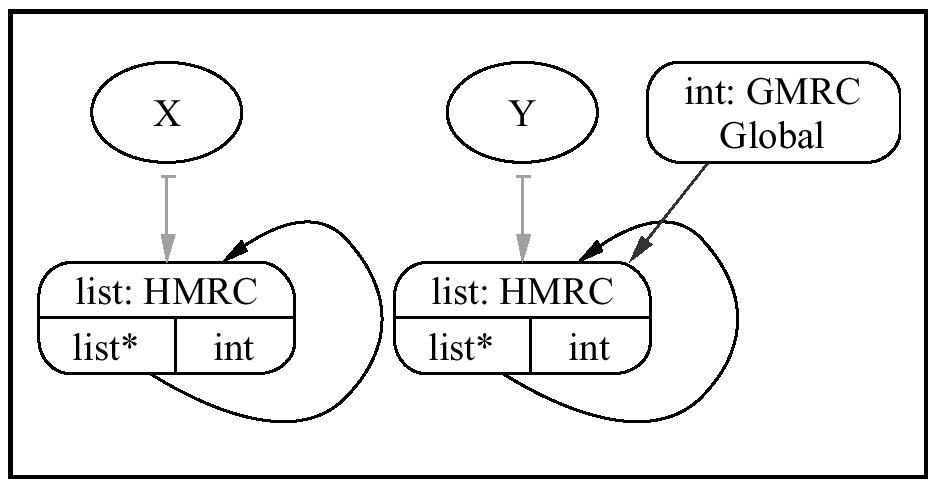
\includegraphics[scale=0.2]{./fig/4.png}
	\end{figure}
\end{frame}

\begin{frame}{Problem}
  Apa is a backend optimize method in LLVM.
  \begin{center}
	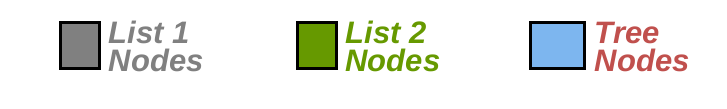
\includegraphics[scale = 0.3]{./fig/1.png}
\end{center}
What the compiler sees
\begin{center}
  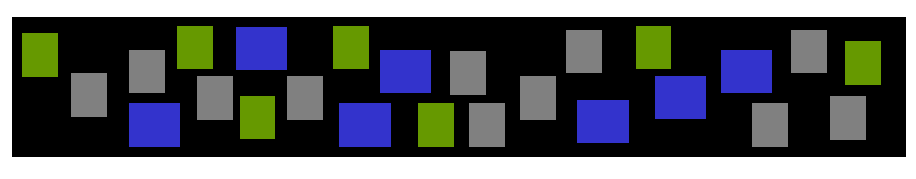
\includegraphics[scale = 0.3]{./fig/2.png}
\end{center}

What we want the program to create and the compiler to see
\begin{center}
  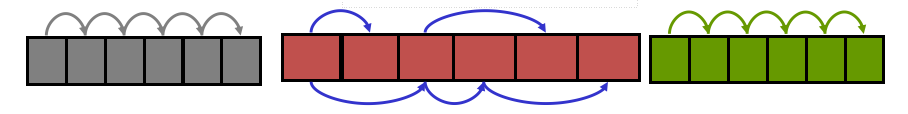
\includegraphics[scale = 0.3]{./fig/3.png}
\end{center}

\end{frame}

\begin{frame}{Problem}
  \begin{itemize}
	  \setlength{\itemsep}{0.5cm}
	\item \textbf{Memory system performance is important!}
	  \begin{itemize}
		\item Fast CPU, slow memory, not enough cache
	  \end{itemize}
	\item	\textbf{“Data structures” are bad for compilers}
	  \begin{itemize}
		\item Traditional scalar optimizations are not enough
		  \item	Memory traffic is main bottleneck for many apps
	  \end{itemize}
	\item \textbf{Fine grain approaches have limited gains:}
	  \begin{itemize}
		\item Prefetching recursive structures is hard
		  \item Transforming individual nodes give limited gains
	  \end{itemize}
  \end{itemize}
\end{frame}

\section{DSA algorithm}

\begin{frame}{Compute Disjoint Data Structure Graphs}
  \begin{itemize}
	  \setlength{\itemsep}{0.5cm}
	\item 
  A significant part in poolalloc is computing disjoint data structure graphs.\\
  \item We use an algorithm called Data Structure Analysis (DSA) to compute these disjoint data structure graphs.\\
\item	\textbf{
Properties of DSA:}
	\begin{itemize}
	  \item context-sensitive(malloc nodes of two distinct lists in a same point)\\
	  \item unification-based(simplification, may-point-to)\\
	  \item field-sensitive(avoid merging the target of unrealted pointer field)
	\end{itemize}
  \end{itemize}
\end{frame}

\begin{frame}{DSA}
  In DSA, the key analysis informations we use is as follows:
  \begin{itemize}
	\item SSA form: assume a low-level code representation with
an infinite set of virtual registers, and a load-store architecture
\item Identification of memory objects: heap objects allocated by malloc, stack objects allocated
by alloca, global variables, and functions;
\item Type information:  we assume that all SSA variables and
memory objects have an associated type.
\item Safety information: our analysis requires that there is
some way to distinguish type-safe and type-unsafe usage of
data values.
  \end{itemize}

\end{frame}

\begin{frame}{Disjoint Data Structure Graph}
  Elements:
  \begin{itemize}
	\item Node
	  \begin{itemize}
		\item each node represents a
typed SSA register or a memory object allocated by the program, or
multiple objects of the same type. 
\item A node is represented by a node
type(new node/alloca node/global node/function node/call node/shadow node/cast node/scalar node)
	  \end{itemize}
	\item Edge 
	  \begin{itemize}
\item 		Each edge in the graph connects a pointer field of one node
(the source field) to a field of another node (the target field).
\item 
	  A pointer field may have edges to multiple targets, i.e.,
edges represent “may-point-to” information.
	  \end{itemize}
  \end{itemize}
\end{frame}

\begin{frame}{Example}
  \begin{figure}[H]
	\centering
	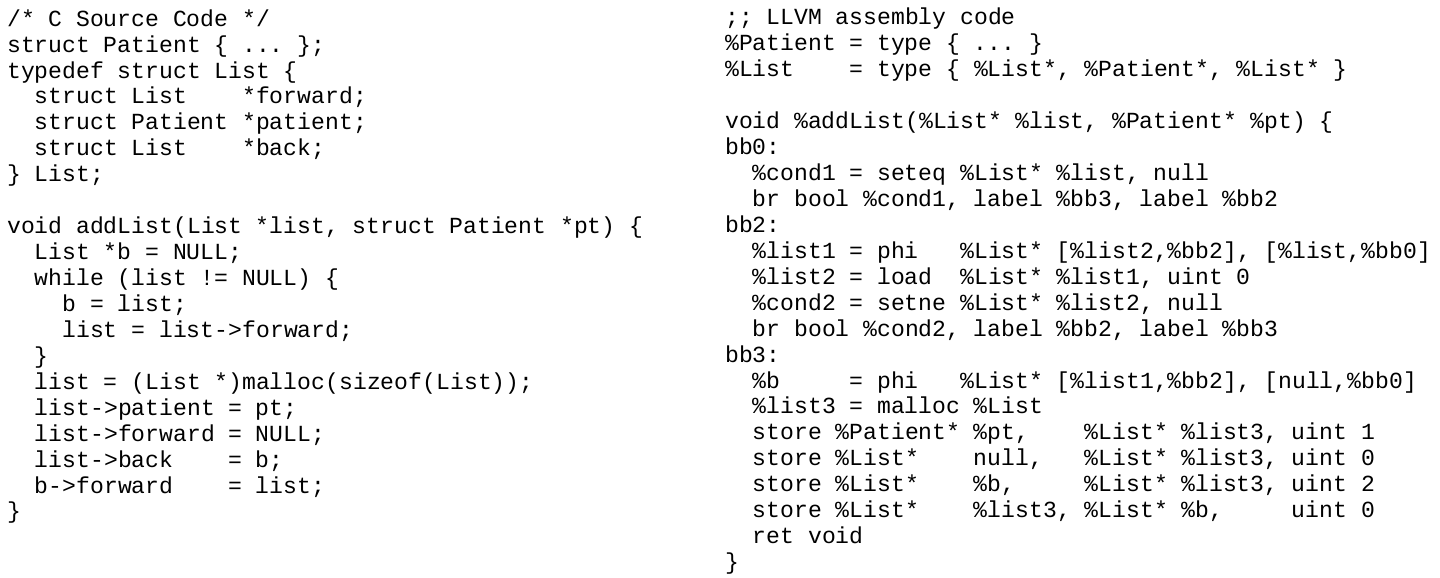
\includegraphics[scale=0.25]{./fig/node.png}
  \end{figure}
\end{frame}

\begin{frame}{Example}
  \textbf{Data Structure Graph} for \emph{addList}:
  \begin{figure}[H]
	\centering
	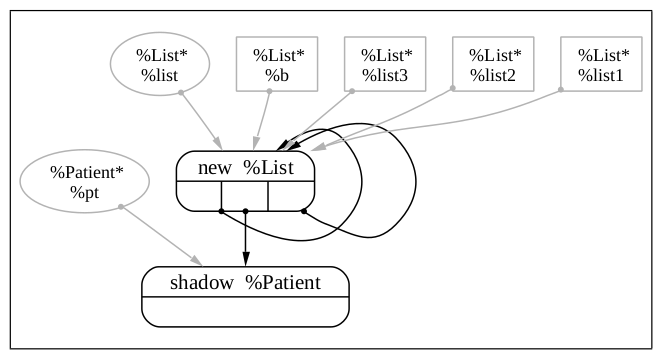
\includegraphics[scale=0.3]{./fig/dd.png}
  \end{figure}
  In our graphs, the dark
rounded objects represent actual memory objects that exist in the
program, whereas the lighter objects represent scalar values in
the function.
\end{frame}

\begin{frame}{Intraprocedural Analysis Algorithm}
  \begin{itemize}
\setlength{\itemsep}{0.5cm}
  \item The intraprocedural graph computation phase is a flow-insensitive analysis that builds a data structure graph without requiring the
code for other functions to be available.

\item The graph construction algorithm is composed of three distinct
phases:
\begin{itemize}
  \item the node discovery phase
	\item the worklist processing phase
	  \item and the graph simplification phase
\end{itemize}
\end{itemize}
\end{frame}

\begin{frame}{Node Discovery Phase}
  \begin{itemize}
	  \setlength{\itemsep}{0.5cm}
	\item Performs a single \textbf{pass} over the function being processed, creating the nodes that make up the graph.
\item The worklist processing phase can only add new shadow nodes and
edges to the graph, so all nodes of other types come from the node
discovery phase.
  \end{itemize}
\end{frame}

\begin{frame}{Worklist processing}
  \begin{itemize}
	\item The worklist contains all of the instructions in the function that use
the SSA values corresponding to the nodes.
\item Processing:
  \begin{algorithm}[H]
	\caption{ProcessWorkList}
	\begin{algorithmic}[1]
	  \WHILE{$WL\neq\varnothing$}
	  \STATE instruction $inst = WL.head$
	  \STATE $WL.$remove($inst$)
	  \STATE $process\ instruction(inst)$
	  \ENDWHILE
	\end{algorithmic}
  \end{algorithm}
\item Worklist processing phase will create shodow nodes and add edges between nodes according to points-to relations.
  \end{itemize}
\end{frame}

\begin{frame}{Graph Simplification}
  \begin{itemize}
	\item Merge indistinguishable nodes(edge points change). Two nodes are considered
	  indistinguishable if they are of the same LLVM type and if there is a field in the data structure graph that points to both nodes..
	  \item Pool allocation actually benefits from graphs that are
merged as much as possible, as long as two disjoint structures are
not unneccesarily merged together.
  \end{itemize}
\end{frame}

\begin{frame}{Interprocedural Closure Algorithm}
  \begin{itemize}
	  \setlength{\itemsep}{0.5cm}
	  \item Local analysis graph is of limited usefulness:
		\begin{itemize}
		  \item Intraprocedural analysis only uses code available in current function.
			\item Most interesting data structures are passed to funcion to construct or manipulate them.
		\end{itemize}
		Therefore, we can not know those datastructures' type, transformation becomes impossible.
%    \item The local analysis graph is of limited usefulness for program
%transformation, because most interesting data structures are passed
%to functions to construct or manipulate them.
%\item Without interprocedural information, it is impossible to transform these functions, because one of
%the called functions may use the data structure in ways not reflected
%in the local data structure graph.
%\item The interprocedural closure algorithm is the process
%of resolving call nodes to the graphs that they represent, propogating interprocedural information from the called functions to
%the caller function’s graphs: when the data structure graphs for the
%called functions are available, the call nodes are eliminated, being
%replaced with the analysis information in the called function graph
%itself.
		\item Interprocedural Closure:
		  \begin{itemize}
			\item Inline information of called funcions to the caller function's graphs.
		  \end{itemize}
  \end{itemize}
\end{frame}

\begin{frame}{Interprocedural Closure Algorithm}
  Special Cases:
  \begin{itemize}
	  \setlength{\itemsep}{0.5cm}
	\item Indirect calls: repeatedly inlining the
called function graphs for each function called by a particular call
node, that is recursively inlining the indirect call.
\item Recursive function: The result of inlining
a function call is memoized in the InlinedFnsSet to avoid infinite
recursion when inlining recursive functions.
\item Mutually recursive function: calculate the interprocedural closure graphs
  in a postorder traversal over the call graph.
  \end{itemize}
\end{frame}

\section{Automatic Pool Allocation}
\begin{frame}{Runtime Support}
  \begin{itemize}
	  \setlength{\itemsep}{0.5cm}
	\item 
  A simple pool allocation runtime library with four
external functions:
\begin{itemize}
  \item poolinit
	\item pooldestroy
	  \item poolalloc
		\item poolfree
\end{itemize}
\item Our pool allocator assumes that a memory pool consists of uniformly sized objects, but can allocate multiple consecutive objects
if needed (for arrays).
\item When pool allocating a complex data structure, each data structure node in the graph
is allocated from a different pool in memory.
  \end{itemize}
\end{frame}

\begin{frame}{Identifying candidate data structures}
  \begin{itemize}
	  \setlength{\itemsep}{0.5cm}
	\item In order to pool allocate a data structure, we must detect the
bounds on the lifetime of the data structure (to allocate and delete
the pools themselves), and determine whether it is safe to pool 
allocate the data structure.
\item Using the data structure graph, we detect data structures whose
lifetimes are bound by a function lifetime, allowing us to allocate
the pool on entry to the function, and deallocate it on exit from the
function.
\item Each function's graph only contains the
  data structures that are acessable by that function, so we identify these candidates by scanning the functions
in the program
  \end{itemize}
\end{frame}

\begin{frame}{Candidate identification algorithm}
  \begin{algorithm}[H]
	\caption{PoolAllocateProgram}
	\begin{algorithmic}[1]
	  \FOR{each function $Fn\in Prog$}
	  \FOR{each disjointdatastructure $DS\in DSGraph(F_n)$} 
	\IF {CallNodes($DS$) $\cup$ CastNodes($DS$) = $\varnothing$}
	\IF {$\neg$ escapes(DS)}
	\STATE {PoolAllocate($Fn, DS$)}
	\ENDIF
	\ENDIF
	\ENDFOR
	\ENDFOR
	\end{algorithmic}
  \end{algorithm}
  %\begin{figure}[H]
  %  \centering
  %  \includegraphics[scale = 0.4]{cand.png}
  %\end{figure}
  \begin{block}{Escape}having globals point to the
structure, or it is returned from the current function.
  \end{block}
\end{frame}

\begin{frame}{Transforming function bodies}
  \begin{algorithm}[H]
	\caption{PoolAllocate}
	\begin{algorithmic}[1]
	  \REQUIRE{funcion $RootFn$, datastructure $DS$}
	  \STATE {$Worklist = \{RootFn$\}}
	  \FOR{each function $Fn\in Worklist$}
	  \FOR{each instruction $I\in$ Instructions($Fn$)} 
	\IF {UsesDataStructure($I, DS)$)}
	\IF {IsMallocOrFree(I)}
	\STATE {ConvertToPoolFunction($I, DS$)}
	\ELSIF{IsCall(I)}
	\STATE {AddPoolArguments($I, DS$)}
	\STATE $Worklist = Worklist \cup $CalledFunction($I$)
	\ENDIF
	\ENDIF
	\ENDFOR
	\ENDFOR
	\end{algorithmic}
  \end{algorithm}
  %\begin{figure}[H]
  %  \centering
  %  \includegraphics[scale = 0.35]{alloc.png}
  %\end{figure}
\end{frame}

\begin{frame}{Transforming funcion bodies}
  \begin{itemize}
	  \setlength{\itemsep}{0.5cm}
	\item $RootFn$'s lifetime bounds the lifetime of $DS$
	  \item The transformation loops over a worklist of functions to process,
transforming each function until the worklist is empty.
\item \textbf{malloc} and \textbf{free} operations referring to the pool allocated
  data structure are changed into calls to the \textbf{poolalloc} and
  \textbf{poolfree} library functions.
  \end{itemize}

\end{frame}
\section{Experiment}

\begin{frame}{Experiment}
  \begin{itemize}
\setlength{\itemsep}{0.5cm}
	\item We use $LLVM\ 3.3$ and $poolalloc\ r192788$ to experiment.
	\item Little resources about how to use $poolalloc$ on the Internet.
	\item Finally, we solved all the problem in using $poolalloc$ thanks to lots of useful help from Prof.Cui and assistant Zhao.
  \end{itemize}
\end{frame}

\begin{frame}{Using DSA}
  $DSA$ roughly works in three distinct phases:
  \begin{itemize}
	  \setlength{\itemsep}{0.5cm}
	\item Local: nodes discovery and create nodes. local analysis is run on each function in the program, creating
separate graphs for each.
	  \item Bottom-Up: run after the local phase. Iterates over the callgraph, callees before
callers, and inlines the callee’s graph into the caller
\item Top-Down: iterates over the callgraph again, this time callers
before callees, and merges nodes in callees when necessary.
  \end{itemize}
\end{frame}

\begin{frame}[fragile]{Using DSA}
  \begin{itemize}
	\item Using $opt$ to load $LLVMDataStructure.so$ and $poolalloc$ libraries to transform on LLVM bytecode.
	  \item Generating bytecode: 
		\begin{lstlisting}
$ clang -emit-llvm -c test.c
\end{lstlisting}
	%$clang\ -emit-llvm\ -c\ test.c$
	  \item DSA analyze(take $Bottom-Up$ analysis as example): 
		\begin{lstlisting}
$ opt -load  /path/to/LLVMDataStructure.so -load 
/path/to/poolalloc.so -analyze  -dsa-bu test.o
\end{lstlisting}
	  \item After last step, it will gennerate .dot files of all the disjoint datastructures. 
	  \item Visualization: using $dot$ program to generate pdf or png file from .dot file.
  \end{itemize}
\end{frame}

\begin{frame}[fragile]{Using poolalloc}
  \begin{itemize}
	\item Optimize: 
	  \begin{lstlisting}
$ opt -load /path/to/LLVMDataStructure.so -load 
/path/to/poolalloc.so -poolalloc test.o > test.o1
\end{lstlisting}
	\item Generate visual bytecode: 
	  \begin{lstlisting}
$ llvm-dis test.o/test.o1
\end{lstlisting}
	\item We can check the differ between not optimized bytecode and optimized bytecode: 
	  \begin{lstlisting}
$ diff test.o.ll test.o1.ll
\end{lstlisting}
	\item Generate executable file: 
	\begin{lstlisting}
$ llc test.o1.ll
$ gcc /path/to/libpoolalloc_rt.a test.o1.s
\end{lstlisting}
  \end{itemize}
\end{frame}

\begin{frame}{Example}
  A simple function \emph{AddList}:
  \begin{figure}[H]
	\centering
	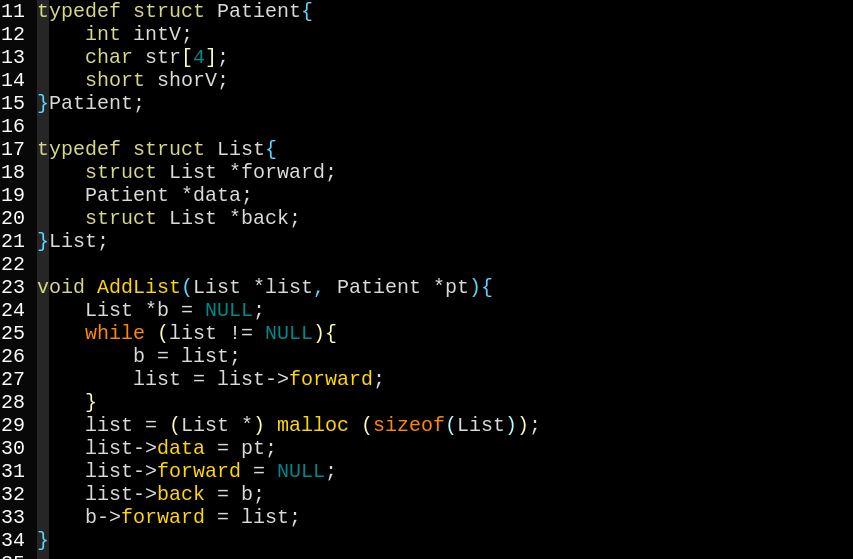
\includegraphics[scale = 0.3]{./fig/src.png}
  \end{figure}
\end{frame}

\begin{frame}{Before poolalloc}
\emph{Objdump} result of binary file compiled with \emph{clang -O3}:
  \begin{figure}[H]
	\centering
	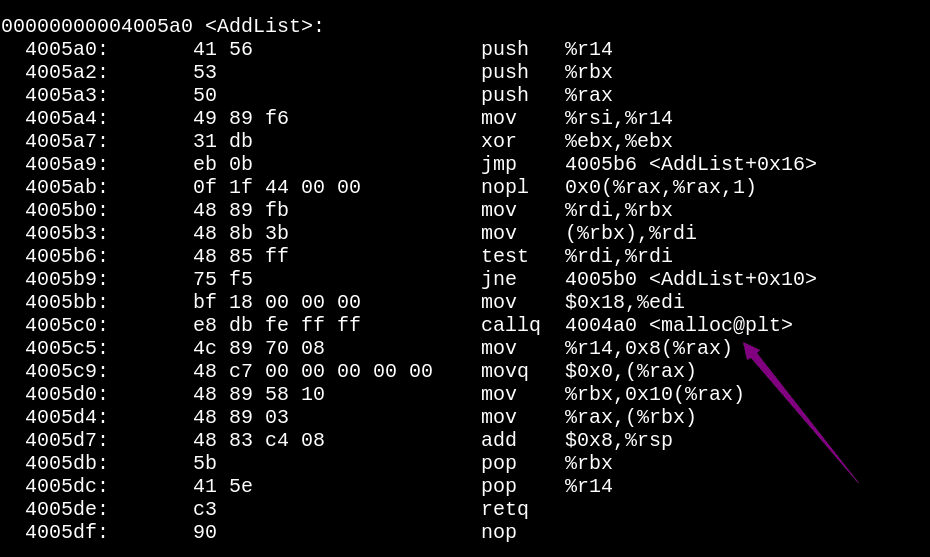
\includegraphics[scale = 0.3]{./fig/nopool.png}
  \end{figure}
\end{frame}

\begin{frame}{After poolalloc}
  \emph{Objdump} result after poolalloc:
  \begin{figure}[H]
	\centering
	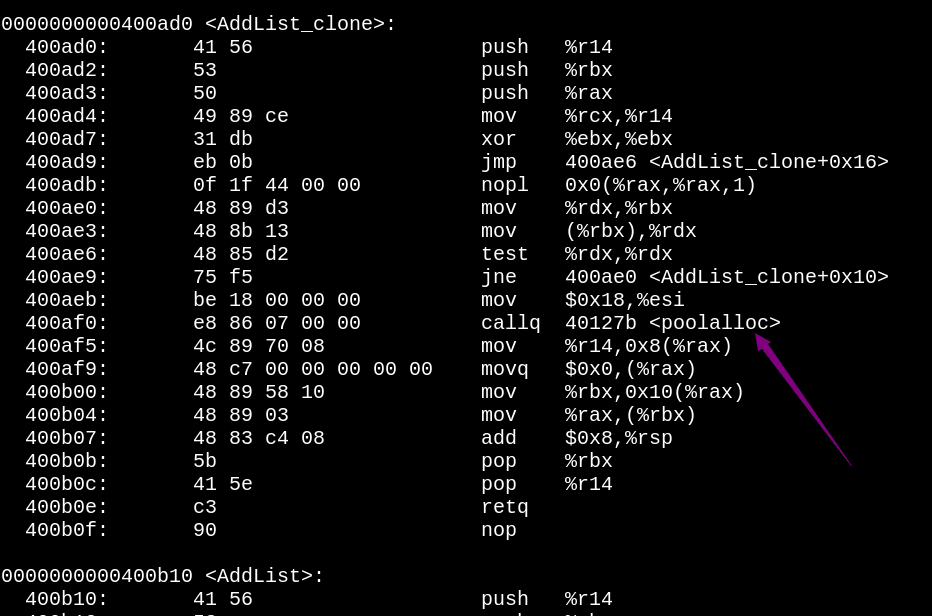
\includegraphics[scale = 0.3]{./fig/pool.png}
  \end{figure}
\end{frame}

\section{Code Analysis}

\begin{frame}{LLVM Pass}{What is LLVM Pass}
  \begin{itemize}
	\item 
  The LLVM Pass Framework is an important part of the LLVM system. Passes perform the transformations and optimizations that make up the compiler, they build the analysis results that are used by these transformations.
\item All LLVM passes are subclasses of the $Pass$ class, which implement functionality by overriding virtual methods inherited from Pass.
  \item Depending on how your pass works, you should inherit from:
	\begin{itemize}
	  \item  $ModulePass$
		\item $FunctionPass$
		  \item  $CallGraphSCCPass$
			\item  $LoopPass$
			  \item  $RegionPass$
				\item $BasicBlockPass$
	\end{itemize}
  \end{itemize}
\end{frame}

\begin{frame}{LLVM Pass}
  \begin{itemize}
\setlength{\itemsep}{0.5cm}
	  \item Passes can be dynamically loaded by the opt tool via its -load option.
	\item Passes are registered with the $RegisterPass$ template. The template parameter is the name of the pass that is to be used on the command line to specify that the pass should be added to a program.
  \end{itemize}
\end{frame}

\begin{frame}
  Example: a simple Pass inherit from the $ModulePass$ which just add a $printf("hello, world.")$ at the beginning of $main$ function if it exists:
  \begin{figure}[H]
	\centering
	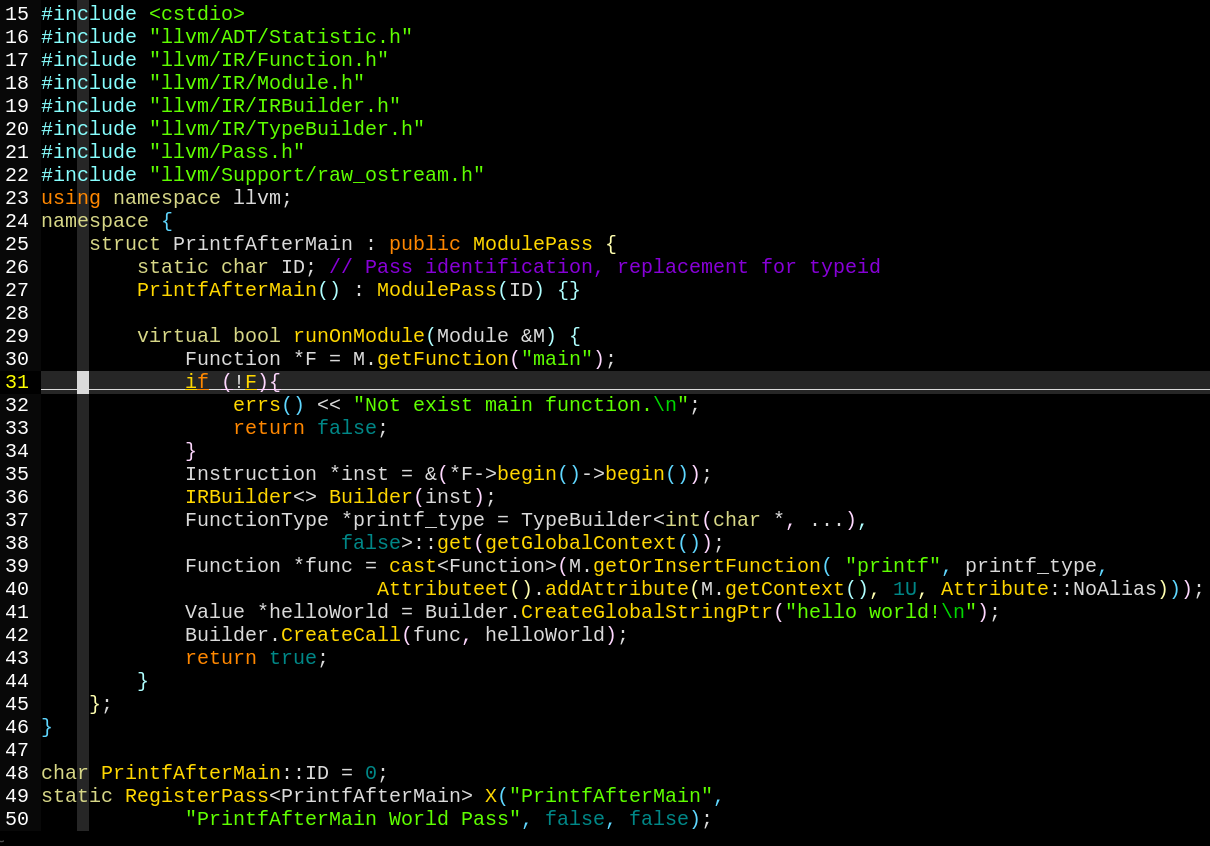
\includegraphics[scale=0.25]{./fig/pass.png}
  \end{figure}
\end{frame}

\begin{frame}{PoolAllocate}
  \begin{itemize}
\setlength{\itemsep}{0.5cm}
	\item file: poolalloc/lib/PoolAllocate/PoolAllocate.cpp
	\item Class PoolAllocate: public PoolAllocateGroup\{//$\dots$\}
	\item Class PoolAllocateGroup: public ModulePass\{//$\dots$\}
	\item Main method: runOnModule(Module \& M)\{//$\dots$\}, it corresponds to the $algorithm$ above(Candidate identification and Transforming function)
  \end{itemize}
\end{frame}

\begin{frame}{bool PoolAllocate: :runOnModule(Module \& M)}
  \begin{block}{}
  \begin{itemize}
\setlength{\itemsep}{0.5cm}
	\item $if (M.begin() = = M.end()) \ return\ false;$ //Module maintains a functions list, Module is empty, so nothing need to do.
	\item $Graphs = \&getAnalysis<\dots>();$ //Accoring to code type, obtain corresponding DSA.
	\item $AddPoolProtypes(\&M)$ // add the pool* prototype to the Module, later we will replace all malloc/free with pool*.
	\item $GlobalPoolCtor = createGlobalPoolCtor(M); SetupGlobalPolls(M);$ // create a global pool and poolalloc all the global DSNodes(reachable from global)
  \end{itemize}
\end{block}
\end{frame}

\begin{frame}{bool PoolAllocate: :runOnModule(Module \& M)}
  \begin{block}{
	continue$\dots$}
  \begin{itemize}
\setlength{\itemsep}{0.5cm}
\item $FindPoolArgs(M);$ // Find the DSNodes for each function that will require pool descriptor arguments to be passed into the function.
	\item Transform functions: Not simply transforming all funcions need to poolalloc.
	\item In order to avoid iterator invalidation errors(random memory errors):
	  \begin{itemize}
		\item Clone all functions which need pool descriptor arguments(Add arguments.)
		  \item Transform all cloned functions or origin functions if the origin has no clone.
		  \item Replace any remaining uses of original functions with the transformed function.
	  \end{itemize}
  \end{itemize}
\end{block}
\end{frame}

\begin{frame}{References}
  \begin{itemize}
	\item \href{https://llvm.org/pubs/2002-06-AutomaticPoolAllocation.html}{Chris Lattner and Vikram Adve. Automatic Pool Allocation for Disjoint Data Structures}
	\item \href{https://llvm.org/pubs/2005-05-21-PLDI-PoolAlloc.html}{Chris Lattner and Vikram Adve. Automatic Pool Allocation: Improving Performance by Controlling Data Structure Layout in the Heap} 
	\item \href{http://llvm.org/docs/WritingAnLLVMPass.html}{Writing an LLVM Pass}
	\item \emph{dsa-manual}
  \end{itemize}
\end{frame}
\end{document}


